Установка, представленная на рис. \ref{img:slits}, позволяет исследовать влияние
дифракции на разрешающую способность оптических инструментов.
Как уже было выяснено, линзы
$O_1$ и
$O_2$ в отсутствие щели
$S_2$ создают
в плоскости
$\Pi$ изображение щели
$S_1$, и это изображение рассматривается
в микроскоп $М$.
Таким образом, нашу
установку можно рассматривать
как оптический инструмент, предназначенный для получения изображения предмета. При этом
коллиматор (щель
$S_1$ и объектив
$O_1$) является
моделью далёкого предмета,
а объектив
$O_2$ и микроскоп
$М$ составляют
зрительную трубу, наведённую на этот предмет.
Если перед объективом
$O_2$ зрительной трубы расположить щель
$S_2$,
то изображение объект
а будет искажено дифракцией на щели
$S_2$. Чем
меньше ширина
$D_0$ этой щели, тем сильнее искажение. Качественной
характеристикой этих искажений мо
жет служить минимальное угловое
расстояние $\phi_{min}$ между объектами (источниками),
которые ещё воспринимаются
как раздельные.

\begin{figure}[h]
  \center{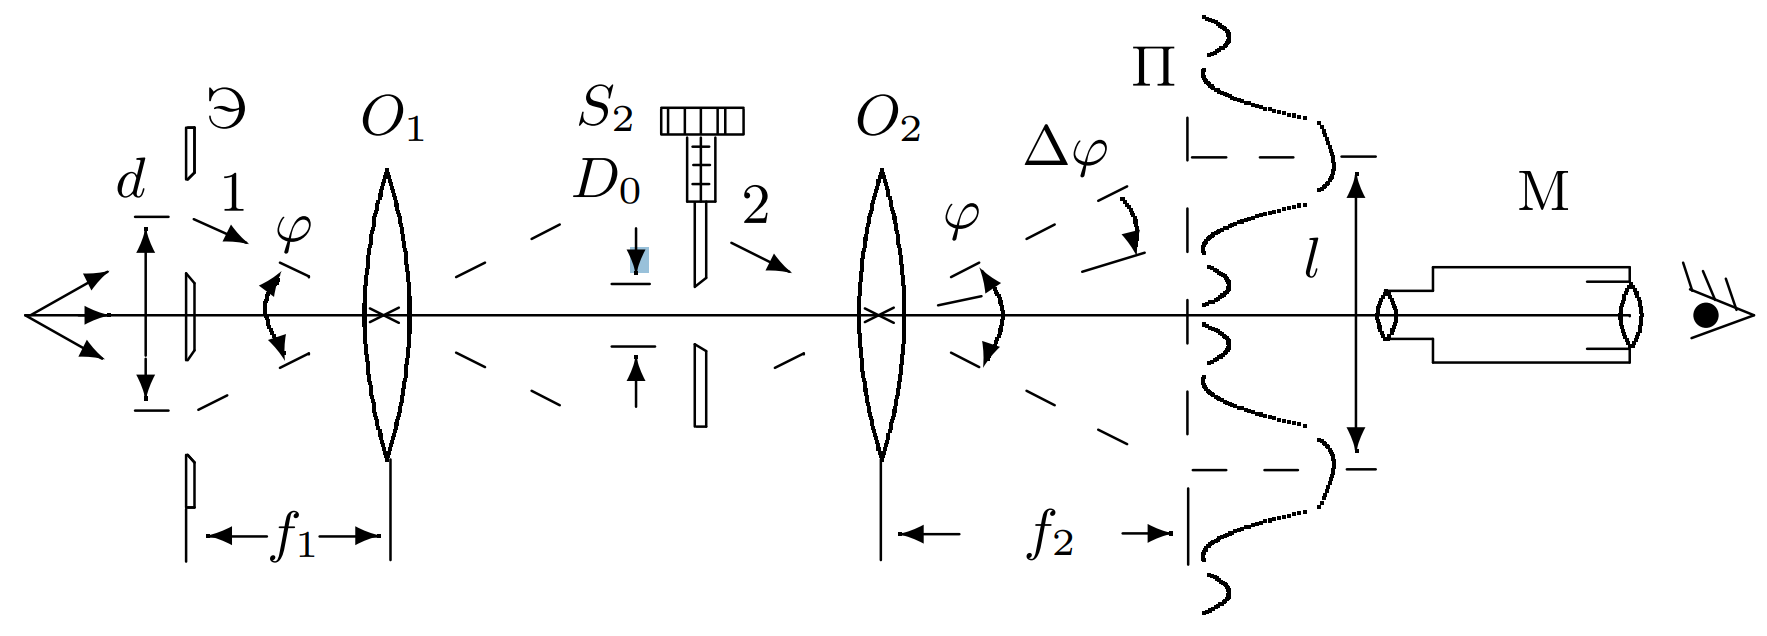
\includegraphics[width=1\linewidth]{fraunres.png}}
  \caption{Схема установки для исследования разрешающей способности оптического инструмента}
  \label{img:fraunres}
\end{figure}

Поместим вместо щели
$S_1$ экран
$Э$ с двумя узкими щелями, расстояние между
которыми равно
$d$ рис. \ref{img:fraunres}.
Тогда на щель
$S_2$ будут падать два параллельных пучка света, составляющих между собой угол
$\phi$, равный (для малых углов)

\begin{equation}
  \phi = \frac{d}{f_1}.
\end{equation}\label{eq:ray_angle}

Параллельные лучи $1$ и $2$, проходящие через центры линз, определяют 
положения изображений двойной щели. 
Согласно законам геометрической оптики расстояние $l$ между изображениями щелей в плоскости
$\Pi$ равно

\begin{equation}
  l = \phi f_2 = d \cdot \frac{f_2}{f_1},
\end{equation}\label{eq:fraun_dist}

а ширина
$\Delta \phi$ каждого изображения определяется дифракцией света на
щели $S_2$. Когда полуширина дифракционного изображения превышает
расстояние между изображениями, то по виду дифракционной
картины
трудно определить, представляет собой источник двойную или одиночную щель. Предельные
условия, при
которых ещё можно различить,
имеем мы дело с одной или двумя щелями, для разных наблюдателей
различны.


\begin{wrapfigure}{r}{0.4\linewidth} % обтекание текстом
  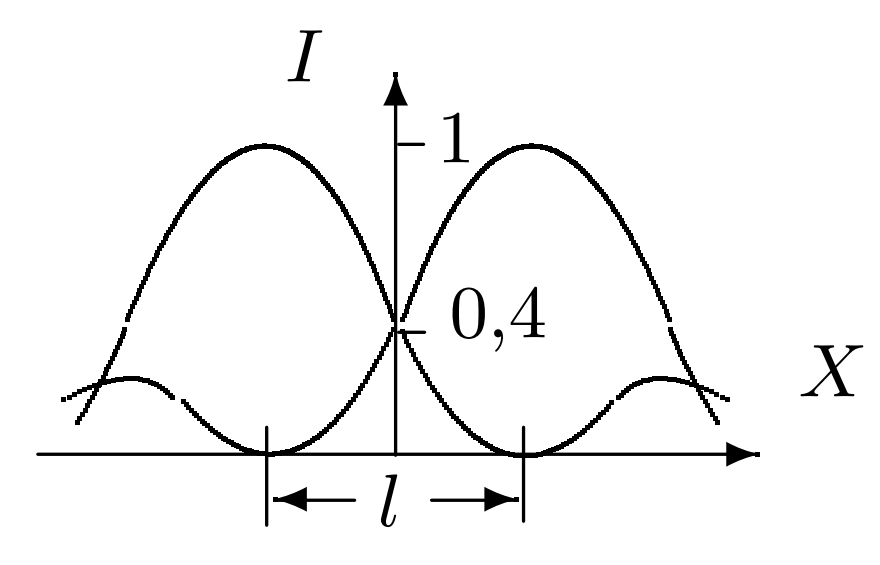
\includegraphics[width=\linewidth]{releus.png}
  \caption{Критерий разрешения по Рэлею}
  \label{img:rele_crit}
\end{wrapfigure}

Для того чтобы исключить связанный
с этим произвол, пользуются обычно критерием Рэлея,
который приблизительно соответствует возможностям визуального наблюдения: изображения считаются различимыми,
когда максимум одного дифракционного пятна совпадает с минимумом другого,
а в условиях нашей задачи ~---~ когда угловая полуширина дифракционного изображения $\lambda/D_0$ совпадает с угловым расстоянием
$\phi= l/f_2$ между изображениями отдельных щелей (рис. \ref{img:rele_crit}):

\begin{equation}
  \frac{\lambda}{D_0} = \frac{l}{f_2} = \frac{d}{f_1}
\end{equation}\label{eq:angle_dist}
